\documentclass[conference]{IEEEtran}
\IEEEoverridecommandlockouts

\usepackage[utf8]{inputenc}
\usepackage[T1]{fontenc}
\usepackage{amsmath,amssymb}
\usepackage{graphicx}
\usepackage{booktabs}
\usepackage{multirow}
\usepackage{siunitx}
\usepackage{xcolor}
\usepackage{url}
\usepackage[hidelinks]{hyperref}
\usepackage{cite}
\usepackage{tikz}
\usetikzlibrary{positioning,arrows.meta}
\usepackage[section]{placeins}
\renewcommand{\topfraction}{0.9}
\renewcommand{\bottomfraction}{0.8}
\renewcommand{\textfraction}{0.07}
\renewcommand{\floatpagefraction}{0.75}
\renewcommand{\dbltopfraction}{0.9}
\renewcommand{\dblfloatpagefraction}{0.75}
\setcounter{topnumber}{3}
\setcounter{bottomnumber}{2}
\setcounter{totalnumber}{6}
\setcounter{dbltopnumber}{2}

\graphicspath{{figures/}}
\sisetup{group-separator={,}, group-minimum-digits=4}
\setlength{\tabcolsep}{4pt}

\begin{document}

\title{Benchmarking Classical Machine Learning for Four-Level Depression Severity Classification from Text: A Leakage-Controlled Study with Clinical-Lexicon and Label-Noise Analyses}

\author{
\IEEEauthorblockN{Raghav Vashisht}
\IEEEauthorblockA{Department of Computer Science and Engineering\\
Chitkara Institute of Engineering (CUIET)\\
Punjab, India}
\and
\IEEEauthorblockN{Aanandit Kanwar}
\IEEEauthorblockA{Department of Computer Science and Engineering\\
Chitkara Institute of Engineering (CUIET)\\
Punjab, India}
\and
\IEEEauthorblockN{Apurav Gautam}
\IEEEauthorblockA{Department of Computer Science and Engineering\\
Chitkara Institute of Engineering (CUIET)\\
Punjab, India}}

\maketitle

% ---------------------------------------------------------------------------
\begin{abstract}
Text that people write online carries measurable signs of depression, and a screening tool built on it must grade severity and explain its decisions. However, the public four-level Depression Severity Levels Dataset contains duplicated and contradictorily labelled posts in 30\% of its rows, and transparent baselines that control for this leakage are rarely reported. In this paper we audit the corpus and benchmark Naive Bayes, Logistic Regression, Random Forest and NB-SVM in five defined experiments, which test Bag-of-Words features, the clinical DSAS lexicon published with the dataset, label-noise filtering by confident learning and a Severe-recall operating point. NB-SVM reaches a macro-F1 of $0.671\pm0.008$ over five splits, a tuned threshold raises Severe recall to 0.82, and the lexicon adds no accuracy but attributes 72\% of Severe predictions to named symptoms. Without the audit, duplicates inflate Logistic Regression and Random Forest by more than six points and reverse the model ranking, while setting aside the 19\% of posts with inconsistent labels lifts macro-F1 to 0.80, which places the performance ceiling in the labels rather than in the models.
\end{abstract}

\begin{IEEEkeywords}
depression severity, natural language processing, bag-of-words, clinical lexicon, label noise, confident learning, data leakage, mental-health screening
\end{IEEEkeywords}

% ---------------------------------------------------------------------------
\section{Introduction}

Depressive disorders affect an estimated 280 million people and are a leading cause of disability worldwide~\cite{who2023depression}. Standardised instruments such as the Beck Depression Inventory (BDI)~\cite{beck1996bdi2,beck1988psychometric} and the PHQ-9~\cite{kroenke2001phq9} grade severity, but they require contact with a professional or a deliberate self-assessment, which stigma and limited mental-health services often prevent. People increasingly describe how they feel on forums and social media, and this text carries measurable linguistic markers of depression~\cite{rude2004language,dechoudhury2013predicting}. Analysing it offers a scalable and non-invasive first step before a formal clinical evaluation, and classical models can do so quickly and transparently.

Most computational work treats depression as a binary label~\cite{dechoudhury2013predicting,coppersmith2014quantifying}, whereas clinical practice is graded: a Mild and a Severe presentation call for different responses, and missing a Severe case costs far more than over-flagging a Mild one. Four-level severity datasets now exist~\cite{naseem2022early,sampath2022dataset,kuas2023dataset}, but three problems limit what results on them mean. Recent work favours deep models and seldom reports classical baselines with a reproducible tuning protocol. Corpora assembled from several sources can contain duplicate and contradictorily labelled posts that fall on both sides of a train/test split, a form of leakage known to inflate reported scores~\cite{kapoor2023leakage,lee2022dedup}, and to our knowledge nobody has measured it for depression-severity text. Finally, screening tools must be auditable, yet the words that push a severity model towards a Severe prediction are rarely reported.

We address these problems with a leakage-controlled study of classical models on the Depression Severity Levels Dataset~\cite{kuas2023dataset}. We first audit the corpus and remove empty, contradictorily labelled and duplicate posts. We then run five experiments that each change one factor: a Bag-of-Words baseline, the clinical lexicon that the dataset authors publish for future work, an NB-SVM classifier, label-noise filtering by confident learning~\cite{northcutt2021confident}, and a decision threshold tuned for Severe recall. Because severity is ordinal, we also report quadratic weighted kappa, and we repeat the main models over five data splits. Table~\ref{tab:scen} lists every experiment and the question it answers.

Our contributions are:
\begin{itemize}
  \item An audit and leakage analysis of the dataset. Duplicates and contradictory labels make up 30\% of the rows and create its apparent class balance; on the uncleaned file, Logistic Regression and Random Forest gain 6.4 to 6.5 macro-F1 points and overtake Naive Bayes, which reverses the true ranking.
  \item A reproducible classical benchmark under clearly defined scenarios. NB-SVM is the strongest and most stable model ($0.671\pm0.008$ over five splits), Naive Bayes is the best Bag-of-Words model (0.652) and trains in under two seconds, and a tuned threshold reaches 0.82 Severe recall.
  \item The first test of the DSAS clinical lexicon published with the dataset, together with a label-noise analysis. The lexicon does not raise accuracy, but it explains 72\% of Severe predictions by named symptoms; removing the 19\% of posts whose labels disagree with the rest of the corpus lifts macro-F1 to 0.80, which shows that label consistency limits performance.
\end{itemize}
All code and results can be regenerated from the public dataset.

% ---------------------------------------------------------------------------
\section{Related Work}

\textbf{Depression detection from user text.} De~Choudhury et al.~\cite{dechoudhury2013predicting} predicted later depression diagnoses from social-media activity, and Coppersmith et al.~\cite{coppersmith2014quantifying} measured mental-health signals on Twitter from self-reported diagnoses. Shared tasks such as CLEF eRisk~\cite{losada2016test} and Reddit corpora~\cite{yates2017depression} formalised early-risk detection, and Guntuku et al.~\cite{guntuku2017detecting} name label quality and generalisability as recurring weaknesses of this work. These studies frame the task as binary or as risk ranking, so they do not tell a screener how severe a case is.

\textbf{Severity-level datasets.} Naseem et al.~\cite{naseem2022early} re-annotated Reddit posts into four severity levels and proposed ordinal classification. Sampath and Durairaj~\cite{sampath2022dataset} released a three-level social-media dataset. The Depression Severity Levels Dataset~\cite{kuas2023dataset} aggregates public corpora into four BDI-aligned levels and was released with HelaDepDet~\cite{priyadarshana2023heladepdet}, a confidence-vector deep model whose authors describe the corpus as well balanced after balancing steps. The dataset authors list a depression lexicon~\cite{cha2022lexicon} as the next enhancement. Neither work audits the aggregated corpus for duplicates or tests the lexicon, which we do in Sections~\ref{sec:audit} and~\ref{sec:lex}.

\textbf{Linguistic markers.} Depressed students use the first-person pronoun ``I'' more often~\cite{rude2004language}, and absolutist words such as ``always'' and ``nothing'' mark depression, anxiety and suicidal ideation~\cite{almosaiwi2018absolute}. Generic stop-word lists delete exactly these words, so we keep them during preprocessing.

\textbf{Classical models and strong linear baselines.} Classical linear and ensemble models remain competitive on short, lexically rich text and are cheaper to train, deploy and explain than transformers~\cite{guntuku2017detecting}. Complement Naive Bayes~\cite{rennie2003tackling}, L1-regularised logistic regression~\cite{tibshirani1996lasso,zou2005elasticnet} and Random Forests~\cite{breiman2001rf} are standard baselines, and NB-SVM~\cite{wang2012baselines}, which scales features by Naive Bayes log-count ratios before a linear classifier, is a strong and cheap text baseline. Severity benchmarks seldom report these models under one tuned protocol, which Experiments~A and~C provide.

\textbf{Leakage, duplication and label errors.} Kapoor and Narayanan~\cite{kapoor2023leakage} document leakage as a common cause of over-optimistic results in ML-based science, and Lee et al.~\cite{lee2022dedup} show that de-duplication changes model behaviour and evaluation. Confident learning~\cite{northcutt2021confident} flags likely label errors from out-of-sample probabilities, and such errors are common even in the test sets of popular benchmarks~\cite{northcutt2021pervasive}. We apply both lenses to depression-severity text, where neither has been measured.

% ---------------------------------------------------------------------------
\section{Method}

\subsection{Overview and Notation}

Fig.~\ref{fig:pipe} shows the pipeline. The corpus is a set of posts $\mathcal{D}=\{(d_i,y_i)\}_{i=1}^{N}$ with severity labels $y_i\in\{0,1,2,3\}$ for Minimal, Mild, Moderate and Severe ($K=4$ classes). After preprocessing, each post $d$ becomes a vector $\mathbf{x}_d\in\mathbb{R}^{|V|}$ over a vocabulary $V$ of unigrams and bigrams, and $x_{t,d}$ is the value for term $t$. A classifier with weights $\mathbf{W}\in\mathbb{R}^{K\times|V|}$ outputs class probabilities $\hat{P}(c\mid\mathbf{x})$, and $\hat{y}$ is the predicted class. $N_c$ is the number of training posts in class $c$. Vectors are bold lowercase and matrices bold uppercase.

\begin{figure}[!htbp]
\centering
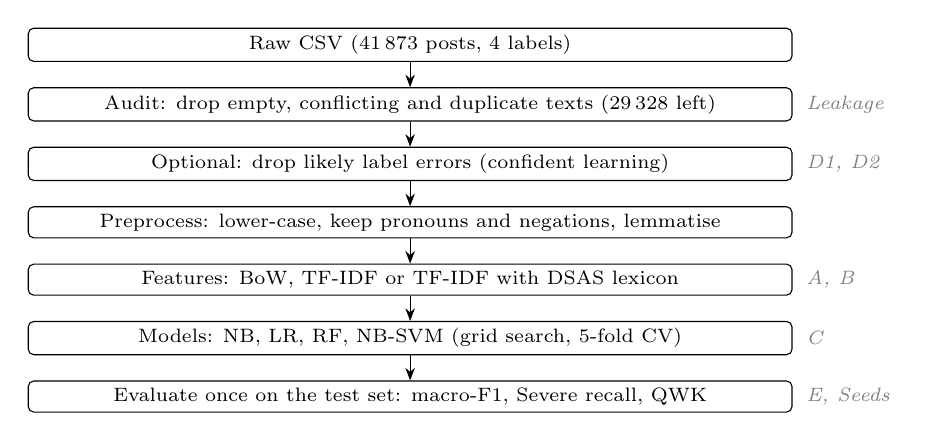
\begin{tikzpicture}[node distance=3.2mm,
  box/.style={draw, rounded corners=2pt, align=center, font=\scriptsize, minimum width=0.8\linewidth, inner sep=2.5pt},
  tag/.style={font=\scriptsize\itshape, text=gray, align=left},
  arr/.style={-{Stealth[length=1.6mm]}}]
\node[box] (raw) {Raw CSV (\num{41873} posts, 4 labels)};
\node[box, below=of raw] (audit) {Audit: drop empty, conflicting and duplicate texts (\num{29328} left)};
\node[box, below=of audit] (noise) {Optional: drop likely label errors (confident learning)};
\node[box, below=of noise] (prep) {Preprocess: lower-case, keep pronouns and negations, lemmatise};
\node[box, below=of prep] (feat) {Features: BoW, TF-IDF or TF-IDF with DSAS lexicon};
\node[box, below=of feat] (model) {Models: NB, LR, RF, NB-SVM (grid search, 5-fold CV)};
\node[box, below=of model] (eval) {Evaluate once on the test set: macro-F1, Severe recall, QWK};
\foreach \a/\b in {raw/audit,audit/noise,noise/prep,prep/feat,feat/model,model/eval} \draw[arr] (\a) -- (\b);
\node[tag, right=0.5mm of audit.east, anchor=west] {Leakage};
\node[tag, right=0.5mm of noise.east, anchor=west] {D1, D2};
\node[tag, right=0.5mm of feat.east, anchor=west] {A, B};
\node[tag, right=0.5mm of model.east, anchor=west] {C};
\node[tag, right=0.5mm of eval.east, anchor=west] {E, Seeds};
\end{tikzpicture}
\caption{Pipeline from the raw file to evaluation. Grey labels mark the stage that each experiment of Table~\ref{tab:scen} changes; all other stages stay as in the baseline.}
\label{fig:pipe}
\end{figure}

\subsection{Dataset and Audit}\label{sec:audit}

The Depression Severity Levels Dataset~\cite{kuas2023dataset} is a single CSV with a \texttt{text} and a \texttt{label} column. The dataset authors align the four labels to BDI score bands: Minimal (0 to 9), Mild (10 to 18), Moderate (19 to 29) and Severe (30 to 63)~\cite{beck1988psychometric}. The labels are annotations of text under the authors' Depression Severity Annotation Schema (DSAS); they are not questionnaire scores from the people who wrote the posts and are not clinical diagnoses. The repository also publishes the DSAS lexicon (Table~\ref{tab:dsas}), which we test in Experiment~B.

Before modelling we audited the corpus (Table~\ref{tab:audit}). Exact duplicates were common, and \num{3053} unique texts carried more than one label. Of these, \num{3028} were labelled both Minimal and Moderate, which points to a systematic mapping difference between source corpora rather than random annotator disagreement. No correct label can be recovered for such texts, so we removed every copy. We collapsed the remaining exact duplicates to one instance and, after preprocessing, dropped 32 posts with no tokens left.

\begin{table}[!htbp]
\centering
\caption{Corpus audit. Each step removes rows from the result of the previous step.}
\label{tab:audit}
\begin{tabular}{lrr}
\toprule
Step & Removed & Remaining \\
\midrule
Raw corpus & -- & \num{41873} \\
Empty text & 14 & \num{41859} \\
Conflicting labels (\num{3053} texts, all copies) & \num{6305} & \num{35554} \\
Exact duplicates & \num{6194} & \num{29360} \\
Empty after preprocessing & 32 & \textbf{\num{29328}} \\
\bottomrule
\end{tabular}
\end{table}

\begin{table}[!htbp]
\centering
\caption{Class distribution of the corpus as distributed and after the audit. Duplication of Moderate posts produced the near-uniform balance of the distributed file.}
\label{tab:classes}
\begin{tabular}{lrrr}
\toprule
Class & As distributed & After audit & Change \\
\midrule
Minimal  & \num{10556} & \num{6280}  & $-40.5\%$ \\
Mild     & \num{10661} & \num{10638} & $-0.2\%$ \\
Moderate & \num{9480}  & \num{1744}  & $-81.6\%$ \\
Severe   & \num{11176} & \num{10666} & $-4.6\%$ \\
\midrule
Total    & \num{41873} & \num{29328} & $-30.0\%$ \\
\bottomrule
\end{tabular}
\end{table}

Individual Moderate posts appear up to 14 times in the distributed file, so the near-uniform class balance of the corpus comes from duplication (Table~\ref{tab:classes}). The audited corpus is imbalanced (Moderate is 5.9\%), and we handle this with class weights and macro-averaged metrics instead of resampling. The class counts in the dataset README (Minimal \num{10549}, Mild \num{10661}, Moderate \num{9473}, Severe \num{11176}) equal the file's counts without its 14 empty rows (7 Minimal, 7 Moderate), so the README describes the same file; it does not mention the duplication.

\subsection{Preprocessing}\label{sec:prep}

We (1)~lower-cased each post and normalised apostrophes, (2)~removed URLs and user mentions, (3)~expanded negative contractions (``can't'' to ``can not'', ``don't'' to ``do not''), (4)~removed non-alphabetic characters, (5)~removed stop words and (6)~lemmatised with WordNet, first as a noun and then as a verb. We started from the scikit-learn English stop list~\cite{pedregosa2011sklearn} and kept the words it would delete that matter for depression: first-person pronouns (\textit{i, me, my, mine, myself, we, us, our}), negations (\textit{no, not, nor, never, none, nobody, nothing, nowhere, neither, cannot}) and the affective words \textit{alone, empty, against, without} and \textit{cry}~\cite{rude2004language,almosaiwi2018absolute}. The default token pattern drops one-letter tokens and would delete ``i'', so we used a pattern that keeps them. After preprocessing, a post has 73.2 tokens on average.

\subsection{Feature Representations}

All representations share one vocabulary setting: unigrams and bigrams, minimum document frequency 5, maximum document frequency 0.90 and at most \num{20000} terms. The vectoriser is fitted inside each cross-validation training fold.

\textbf{Bag-of-Words (BoW), Experiment A,} uses raw counts, $x_{t,d}=\mathrm{tf}(t,d)$.

\textbf{TF-IDF}, used inside Experiments B and C, re-weights counts by smoothed inverse document frequency~\cite{salton1988term} and L2-normalises each post:
\begin{equation}
\mathrm{idf}(t)=\ln\frac{1+N}{1+\mathrm{df}(t)}+1,\qquad
x_{t,d}=\frac{\mathrm{tf}(t,d)\,\mathrm{idf}(t)}{\lVert \mathbf{x}_d\rVert_2},
\label{eq:tfidf}
\end{equation}
where $\mathrm{df}(t)$ is the number of training posts that contain $t$.

\textbf{DSAS lexicon, Experiment B.} The lexicon maps 11 depression criteria $k$ to keyword sets $L_k$ (Table~\ref{tab:dsas}). We pass each keyword through the same preprocessing as the posts, so \textit{broken} becomes \textit{break} and \textit{killmyself} becomes \textit{kill myself}. Variant B1 appends one feature per criterion to the TF-IDF vector,
\begin{equation}
s_{k,d}=\log\big(1+n_{k,d}\big),\qquad k=1,\dots,11,
\label{eq:sym}
\end{equation}
where $n_{k,d}$ counts whole-word matches of $L_k$ in post $d$. Variant B2 first adds the WordNet synonyms~\cite{miller1995wordnet} of every one-word keyword, which grows the lexicon from 42 to 291 unique terms, multiplies the TF-IDF columns of lexicon terms by $w=2$ before L2 normalisation, and then appends the counts of Eq.~\eqref{eq:sym} from the expanded lexicon. B1 tells the model how often each symptom is mentioned, and B2 also doubles the weight of symptom words.

\begin{table}[!htbp]
\centering
\caption{DSAS lexicon as published in the dataset repository~\cite{kuas2023dataset}, after Cha et al.~\cite{cha2022lexicon}. Experiment~B uses it as features and for symptom-level explanations.}
\label{tab:dsas}
\footnotesize
\begin{tabular}{p{0.32\linewidth}p{0.58\linewidth}}
\toprule
DSAS criterion & Keywords \\
\midrule
Depressed mood & sadness, anger, bored, hurt, nervousness, moody, emotional \\
Loss of interest & discomfort, unhappy, no-focus, disturbed \\
Appetite change & loss of appetite, overeating, weight loss \\
Sleep change & light sleep, waking up early, short sleep, dreamy \\
Fatigue & bored, useless, isolation, low interaction, fatigue \\
Restlessness & uneasiness, instability \\
Anxiety & stress, pain \\
Worthlessness & useless, hopeless, helpless, lonely \\
Guilt & low self-esteem \\
Poor concentration & hesitate, tired \\
Suicidal thoughts & long-term grief, hopelessness, end-of-my-life, die, suicide, killmyself, suicidal, broken, worthless, self-harm \\
\bottomrule
\end{tabular}
\end{table}

\subsection{Classifiers}

\textbf{Naive Bayes (NB).} Multinomial NB predicts
\begin{equation}
\hat{y}=\arg\max_c\Big[\log P(c)+\sum_t x_{t}\log\theta_{c,t}\Big],\quad
\theta_{c,t}=\frac{N_{c,t}+\alpha}{N_c+\alpha|V|},
\label{eq:nb}
\end{equation}
where $N_{c,t}$ is the count of term $t$ in class $c$. Complement NB~\cite{rennie2003tackling} estimates $\theta$ from all classes except $c$, which is more stable under class imbalance; the grid search chooses between the two variants.

\textbf{Logistic Regression (LR).} Multinomial LR models $\hat{P}(c\mid\mathbf{x})=\exp(\mathbf{w}_c^\top\mathbf{x}+b_c)/\sum_k\exp(\mathbf{w}_k^\top\mathbf{x}+b_k)$ and minimises the class-weighted cross-entropy with an elastic-net penalty~\cite{zou2005elasticnet}:
\begin{equation}
\begin{split}
\mathcal{L}(\mathbf{W})={}&-\sum_i s_{y_i}\log \hat{P}(y_i\mid\mathbf{x}_i)\\
&+\frac{1}{C}\Big[\rho\lVert \mathbf{W}\rVert_1+\frac{1-\rho}{2}\lVert \mathbf{W}\rVert_2^2\Big],
\end{split}
\label{eq:lr}
\end{equation}
with balanced class weights $s_c=N/(K N_c)$. Setting $\rho=1$ gives the L1 (lasso) penalty~\cite{tibshirani1996lasso}, which sets uninformative coefficients to zero. We use the SAGA solver~\cite{defazio2014saga}, which supports L1 and elastic-net penalties on sparse input, with a tolerance of $10^{-3}$ or at most 100 epochs. SAGA converges slowly on raw counts, so for BoW features we rescale each column to $[0,1]$ with a max-absolute scaler, which keeps the matrix sparse.

\textbf{Random Forest (RF).} An ensemble of CART trees, each grown on a bootstrap sample with $\sqrt{|V|}$ candidate features per split, predicts by majority vote~\cite{breiman2001rf}. Splits minimise Gini impurity $G=1-\sum_c p_c^2$, and a feature's importance is its total weighted impurity decrease. We apply balanced class weights.

\textbf{NB-SVM, Experiment C.} Following Wang and Manning~\cite{wang2012baselines}, for each class $c$ we scale the TF-IDF features by the Naive Bayes log-count ratio
\begin{equation}
\mathbf{r}_c=\log\frac{(\mathbf{p}_c+\alpha)/\lVert\mathbf{p}_c+\alpha\rVert_1}{(\mathbf{q}_c+\alpha)/\lVert\mathbf{q}_c+\alpha\rVert_1},
\label{eq:nbsvm}
\end{equation}
where $\mathbf{p}_c$ and $\mathbf{q}_c$ sum the feature vectors of training posts inside and outside $c$ and $\alpha=1$. A class-weighted binary logistic regression is fitted on $\mathbf{x}\odot\mathbf{r}_c$ for each class, and the class with the highest score wins. Naive Bayes thus decides which words carry class information, and logistic regression learns how much each one should count.

\subsection{Label-Noise Detection, Experiment D}

We use a simplified form of confident learning~\cite{northcutt2021confident}. Each post receives out-of-fold probabilities $\hat{P}_{i,c}$ from models that never saw it in training: a TF-IDF logistic regression and a Complement NB, averaged, over five stratified folds. With the per-class threshold $\tau_c=\frac{1}{N_c}\sum_{i:y_i=c}\hat{P}_{i,c}$, post $i$ is flagged as a likely label error when
\begin{equation}
\hat{y}_i\neq y_i,\qquad \hat{P}_{i,\hat{y}_i}\ge\tau_{\hat{y}_i},\qquad \hat{P}_{i,y_i}<\tau_{y_i},
\label{eq:cl}
\end{equation}
that is, when the models confidently prefer another class and give the assigned label less than its usual confidence. Variant D1 removes flagged posts from the training set only and tests on the untouched test set. Variant D2 removes flagged posts from the whole audited corpus before splitting, which estimates performance when labels are internally consistent.

\subsection{Severe Operating Point, Experiment E}

A screening tool may accept more false alarms to miss fewer Severe cases. We multiply the predicted Severe probability by a factor $\lambda\ge1$ and choose the smallest $\lambda$ (in steps of 0.05, up to 6) for which out-of-fold Severe recall on the training set reaches 0.80. We then apply that $\lambda$ once to the test set.

\subsection{Symptom-Level Explanations}

Because LR is linear, its score for the predicted class $\hat{y}$ splits exactly into parts. The contribution of DSAS criterion $k$ to post $d$ is
\begin{equation}
e_{k,d}=\sum_{t\in V_k} w_{\hat{y},t}\,x_{t,d},
\label{eq:expl}
\end{equation}
where $V_k$ contains the vocabulary n-grams that include a term of $L_k$. A positive $e_{k,d}$ means that criterion $k$ pushed the post towards its predicted class.

\subsection{Experimental Scenarios}\label{sec:scen}

Table~\ref{tab:scen} defines every experiment. Experiments B to E reuse the configuration that the grid search selected for the reference model, so each result differs from its reference in exactly one factor.

\begin{table*}[!t]
\centering
\caption{Experimental scenarios. Each scenario changes one factor relative to its reference; a dash means ``as in Experiment A''.}
\label{tab:scen}
\footnotesize
\begin{tabular}{lp{0.2\linewidth}p{0.17\linewidth}p{0.13\linewidth}p{0.35\linewidth}}
\toprule
ID & Data & Features & Models & Question answered \\
\midrule
A & Audited corpus, seed-42 split & BoW & NB, LR, RF & How well do classical models do on clean data? (baseline) \\
B & -- & TF-IDF with DSAS lexicon (B1, B2) & NB, LR, RF & Does the dataset's clinical symptom lexicon help? \\
C & -- & TF-IDF & NB-SVM & Does combining NB word weights with LR help? \\
D1 & Likely label errors removed from the training set & TF-IDF or BoW & LR, NB, NB-SVM & Does cleaning training labels help on the original test set? \\
D2 & Likely label errors removed from the whole corpus & BoW, TF-IDF & NB, LR, RF, NB-SVM & What can the models reach when labels are consistent? \\
E & -- & as in A to C & NB, LR, NB-SVM & Can a model catch 80\% of Severe posts, and at what cost? \\
Leakage & Corpus as distributed & BoW & NB, LR, RF & How much do duplicates distort scores? \\
Seeds & Five stratified splits & as in A and C & NB, LR, RF, NB-SVM & Are the results stable across splits? \\
\bottomrule
\end{tabular}
\end{table*}

% ---------------------------------------------------------------------------
\section{Experimental Setup}

\textbf{Data and splits.} We split the audited corpus 80/20 into training (\num{23462} posts) and test (\num{5866} posts) sets, stratified by class, with seed 42. The robustness runs repeat this with seeds 42 to 46.

\textbf{Tuning.} For each model we ran an exhaustive grid search (Table~\ref{tab:grid}) with stratified five-fold cross-validation on the training set only and selected the configuration with the highest mean macro-F1. The vectoriser is part of the cross-validated pipeline, so vocabulary and IDF statistics never see validation or test posts. We refitted the selected configuration on the full training set and evaluated it once on the test set.

\begin{table}[!htbp]
\centering
\caption{Hyper-parameter grids searched with stratified five-fold cross-validation on the training set.}
\label{tab:grid}
\begin{tabular}{p{0.17\linewidth}p{0.6\linewidth}r}
\toprule
Model & Hyper-parameters & Configs \\
\midrule
NB & variant $\in$ \{Multinomial, Complement\}; $\alpha\in\{0.1,0.5,1.0\}$ & 6 \\
LR & $C\in\{0.1,1,10\}$; $\rho\in\{1.0,0.5\}$; SAGA; balanced weights & 6 \\
RF & trees $\in\{100,300,500\}$; max depth $\in\{20,50,100\}$; min split $\in\{2,5,10\}$; $\sqrt{p}$ features; balanced weights & 27 \\
NB-SVM & $C\in\{1,4,10\}$; balanced weights ($C=1$ selected) & 3 \\
\bottomrule
\end{tabular}
\end{table}

\textbf{Metrics.} We report accuracy, macro-averaged precision, recall and F1, and Severe recall, the share of truly Severe posts predicted as Severe. Severe recall is the critical screening metric because a missed Severe case is the most harmful error. Severity is ordinal, so we also report quadratic weighted kappa (QWK)~\cite{cohen1968weighted},
\begin{equation}
\kappa=1-\frac{\sum_{i,j}(i-j)^2 O_{ij}}{\sum_{i,j}(i-j)^2 E_{ij}},
\label{eq:qwk}
\end{equation}
where $O$ is the confusion matrix and $E$ the matrix expected by chance. QWK is 1 for perfect agreement and 0 for chance, and it penalises a Minimal-for-Severe error nine times more than an error between neighbouring levels.

\textbf{Leakage run.} To measure the effect of duplicates and conflicting labels, we re-ran all three Experiment~A models on the corpus as distributed (\num{41785} posts after removing empty texts): Naive Bayes with its full grid search, and LR and RF with their selected configurations.

\textbf{Compute.} All experiments ran on a laptop with an 8-core arm64 CPU and 8~GB RAM, with Python~3.9 and scikit-learn 1.6.1.

% ---------------------------------------------------------------------------
\section{Results}

\subsection{Baseline, Experiment A}

\begin{table*}[!t]
\centering
\caption{Experiment A: test-set performance of the best configuration of each model on the audited corpus with BoW features (seed-42 split). Bold marks the best value in each column.}
\label{tab:metrics}
\begin{tabular}{llrrrrrrrl}
\toprule
Features & Model & Acc. & Macro-P & Macro-R & Macro-F1 & Severe-R & QWK & CV F1 ($\pm$sd) & Selected configuration \\
\midrule
BoW & Naive Bayes & \textbf{0.680} & \textbf{0.645} & \textbf{0.663} & \textbf{0.652} & \textbf{0.703} & \textbf{0.561} & 0.651 $\pm$ 0.006 & Multinomial, $\alpha$=0.5 \\
BoW & Logistic Regression & 0.640 & 0.593 & 0.625 & 0.603 & 0.602 & 0.489 & 0.610 $\pm$ 0.010 & $C$=1, $\rho$=1 \\
BoW & Random Forest & 0.656 & 0.624 & 0.605 & 0.609 & 0.623 & 0.522 & 0.624 $\pm$ 0.006 & 500 trees, depth 100, split 10 \\
\bottomrule
\end{tabular}
\end{table*}

\begin{figure}[!htbp]
\centering
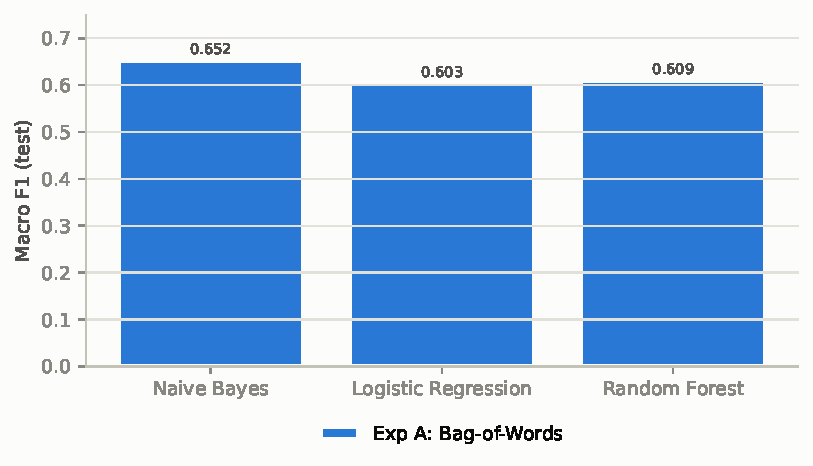
\includegraphics[width=0.85\linewidth]{figA_macro_f1}
\caption{Experiment A: test-set macro-F1 of Naive Bayes, Logistic Regression and Random Forest with BoW features on the audited corpus.}
\label{fig:f1}
\end{figure}

On BoW features Naive Bayes is the best model on every metric (Table~\ref{tab:metrics}, Fig.~\ref{fig:f1}): macro-F1 0.652 against 0.609 for RF and 0.603 for LR, and QWK 0.561 against 0.522 and 0.489. This fits the multinomial model, which describes exactly the word counts that BoW provides. Cross-validated macro-F1 lies within 2.2 points of the test value for every model, so selection did not overfit the split. RF fits its training folds almost perfectly (training macro-F1 0.98) without generalising better than the linear models, and its selected configuration (500 trees, depth 100) sits at the edge of the grid; we did not explore larger forests.

\begin{figure}[!htbp]
\centering
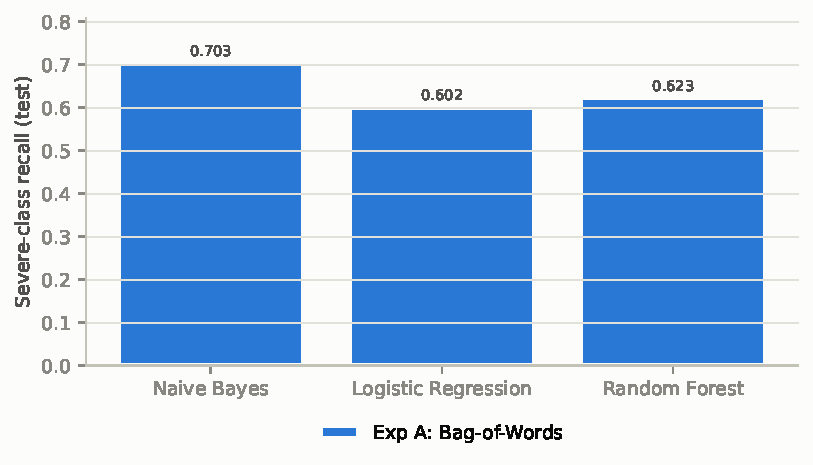
\includegraphics[width=0.85\linewidth]{figA_severe_recall}
\caption{Experiment A: Severe recall, the share of truly Severe test posts predicted as Severe, for each model with BoW features.}
\label{fig:severe}
\end{figure}

Naive Bayes also recalls the most Severe posts, 0.703 against 0.623 for RF and 0.602 for LR (Fig.~\ref{fig:severe}). All three models send most missed Severe posts to Mild (22 to 27\% of true Severe posts) rather than to Minimal (4 to 14\%) or Moderate (2 to 3\%).

\subsection{Error Analysis}

\begin{figure*}[!t]
\centering
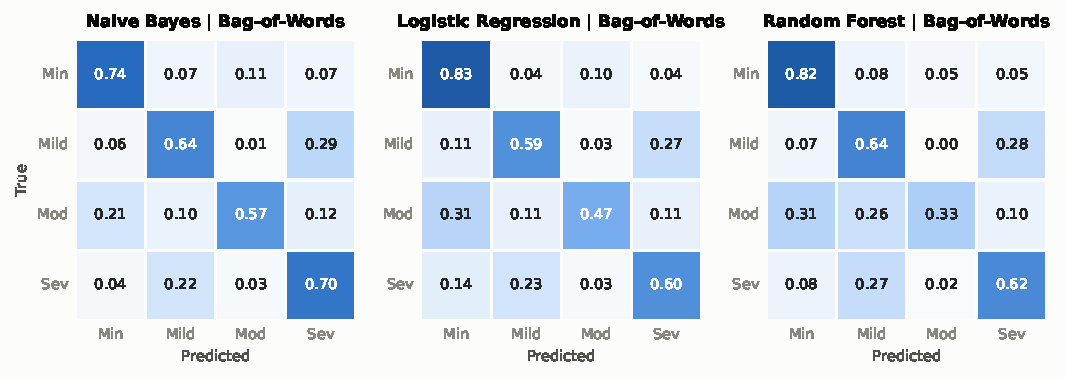
\includegraphics[width=0.75\linewidth]{fig2_confusion_matrices}
\caption{Experiment A: row-normalised confusion matrices on the test set. Cell $(i,j)$ is the share of true class $i$ predicted as class $j$ (Min = Minimal, Mod = Moderate, Sev = Severe). The large Mild-to-Severe and Severe-to-Mild cells skip a level.}
\label{fig:cm}
\end{figure*}

Errors do not concentrate between neighbouring levels (Fig.~\ref{fig:cm}). For every model, one of the two largest errors is Mild predicted as Severe (27 to 29\% of true Mild posts), and the reverse error is almost as large. Mild and Severe are two levels apart, so this pattern fits label noise or source-specific labelling conventions better than genuinely borderline posts. Moderate is the hardest class (per-class F1 0.40 to 0.50): it is the smallest class after the audit, and 21 to 31\% of its posts are predicted as Minimal, the same pair that the audit found in \num{3028} conflicting texts. Experiment~D tests the label-noise explanation directly.

\subsection{Leakage}

\begin{table}[!htbp]
\centering
\caption{Macro-F1 of the Experiment A models on the audited corpus and on the corpus as distributed. On the distributed file 30\% of test posts have an exact copy in the training set.}
\label{tab:leak}
\begin{tabular}{llrrr}
\toprule
Features & Model & Audited & As distributed & $\Delta$ (points) \\
\midrule
BoW & Naive Bayes & 0.652 & 0.637 & $-1.5$ \\
BoW & Logistic Regression & 0.603 & 0.669 & $+6.5$ \\
BoW & Random Forest & 0.609 & 0.673 & $+6.4$ \\
\bottomrule
\end{tabular}
\end{table}

On the corpus as distributed, 30.0\% of test posts have an exact copy in the training set. Naive Bayes loses 1.5 macro-F1 points, while LR and RF gain 6.5 and 6.4 points and overtake it (Table~\ref{tab:leak}). Two effects act in opposite directions. Duplicates shared between the training and test sets let a model recall answers it has already seen, and RF, which nearly memorises its training data, and LR profit most. The \num{3053} contradictorily labelled texts also enter the test set, where at most one of their labels can be predicted correctly, which lowers every score. The net effect depends on the model, so scores on the distributed file cannot be compared with scores on clean data, and on this corpus they reverse the ranking of the models.

\subsection{Clinical Lexicon, Experiment B}\label{sec:lex}

\begin{table}[!htbp]
\centering
\caption{Experiment B on the seed-42 split. The reference rows use the same models with TF-IDF and no lexicon; $\Delta$F1 is the change from the reference in macro-F1 points.}
\label{tab:lex}
\begin{tabular}{llrrr}
\toprule
Features & Model & Macro-F1 & Severe-R & $\Delta$F1 \\
\midrule
Reference (no lexicon) & NB & 0.602 & 0.690 & -- \\
                       & LR & 0.661 & 0.677 & -- \\
                       & RF & 0.598 & 0.624 & -- \\
\midrule
B1: symptom features & NB & 0.591 & 0.704 & $-1.1$ \\
                       & LR & 0.659 & 0.647 & $-0.1$ \\
                       & RF & 0.604 & 0.632 & $+0.6$ \\
\midrule
B2: weighted, expanded & NB & 0.589 & 0.688 & $-1.2$ \\
                       & LR & 0.660 & 0.646 & $-0.1$ \\
                       & RF & 0.604 & 0.626 & $+0.6$ \\
\bottomrule
\end{tabular}
\end{table}

The DSAS lexicon does not improve classification (Table~\ref{tab:lex}). Macro-F1 changes by $-1.2$ to $+0.6$ points, which is within the split-to-split variation in Table~\ref{tab:seeds}, and LR loses 3 points of Severe recall. The decisive lexicon terms (\textit{suicide}, \textit{die}, \textit{suicidal}) are already in the vocabulary, so the classifier learns their weight from the data without help. Coverage is also low: 53.1\% of posts contain any lexicon term, and the appetite, sleep, restlessness and guilt criteria each occur in fewer than 0.5\% of posts in every class (Fig.~\ref{fig:sym}, left).

\begin{figure*}[!t]
\centering
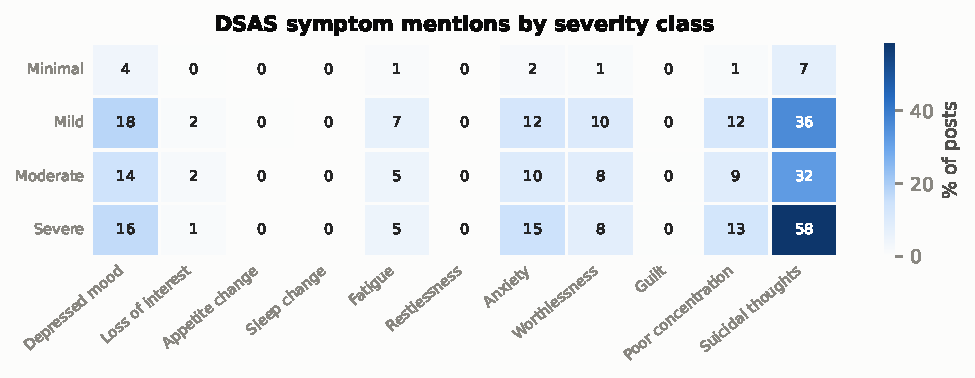
\includegraphics[width=0.49\linewidth]{fig6_symptom_profile}\hfill
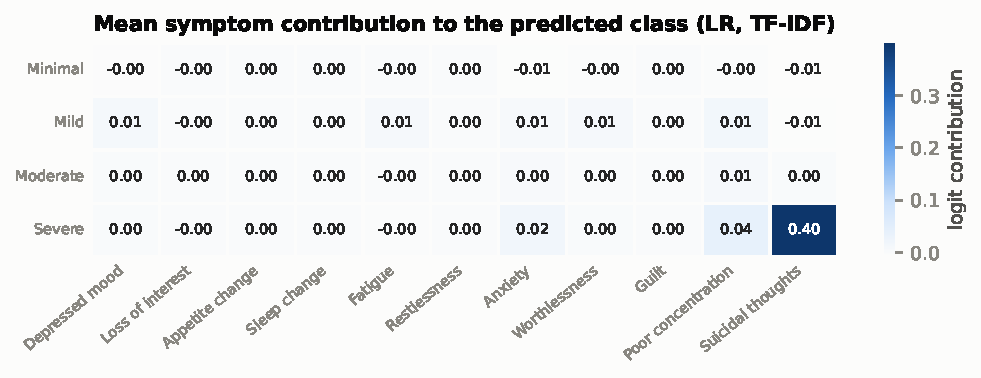
\includegraphics[width=0.49\linewidth]{fig8_symptom_contribution}
\caption{DSAS symptoms by severity class. Left: share of posts in each class of the audited corpus that mention each criterion. Right: mean contribution $e_{k,d}$ (Eq.~\ref{eq:expl}) of each criterion to the predicted-class score of the TF-IDF LR on the test set, grouped by predicted class.}
\label{fig:sym}
\end{figure*}

The lexicon is more useful for explaining predictions. Suicidal-thought terms appear in 58.4\% of Severe posts, but also in 35.9\% of Mild, 31.9\% of Moderate and 7.4\% of Minimal posts (Fig.~\ref{fig:sym}, left), another sign of how close the Mild and Severe annotations are. With the decomposition of Eq.~\eqref{eq:expl}, 72.4\% of Severe predictions can be traced to at least one criterion with a positive contribution, and for 58.3\% of them the largest contributor is suicidal thoughts (Fig.~\ref{fig:sym}, right). Each flagged post therefore comes with a reason that a clinician can check, for example a Severe prediction driven mainly by suicidal-thought and poor-concentration terms.

\subsection{NB-SVM, Experiment C, and Ablation}

\begin{table}[!htbp]
\centering
\caption{Ablation on the original seed-42 test set. Indented rows add one component to the row above them.}
\label{tab:abl}
\begin{tabular}{lrrr}
\toprule
Setup & Macro-F1 & Severe-R & QWK \\
\midrule
Experiment A best (NB, BoW) & 0.652 & 0.703 & 0.561 \\
\quad + training-label cleaning (D1) & 0.648 & 0.702 & 0.557 \\
LR, TF-IDF (reference) & 0.661 & 0.677 & 0.573 \\
\quad + DSAS symptom features (B1) & 0.659 & 0.647 & 0.566 \\
\quad + training-label cleaning (D1) & 0.655 & 0.651 & 0.562 \\
NB-SVM, TF-IDF (C) & 0.659 & 0.640 & 0.568 \\
\quad + training-label cleaning (D1) & \textbf{0.665} & 0.665 & \textbf{0.579} \\
\bottomrule
\end{tabular}
\end{table}

On the seed-42 split NB-SVM (0.659) matches the TF-IDF LR reference (0.661) and beats the best Experiment~A model (0.652) (Table~\ref{tab:abl}). Over five splits its lead is clearer (Table~\ref{tab:seeds}): $0.671\pm0.008$, the highest macro-F1 and QWK of all models. It trains in 5.6~s, against 107~s for the TF-IDF LR. Each component in Table~\ref{tab:abl} changes macro-F1 by at most 0.6 points, so none of them explains the remaining errors; Experiment~D points to the labels instead.

\subsection{Label Noise, Experiment D}

The detector of Eq.~\eqref{eq:cl} flags 18.5\% of training posts (\num{4352}: 534 Minimal, \num{1701} Mild, 319 Moderate, \num{1798} Severe). Removing them from the training set only (D1) changes test macro-F1 by $-0.6$ to $+0.6$ points (Table~\ref{tab:abl}), because the test labels contain the same inconsistencies.

Applied to the whole audited corpus (D2), the detector flags \num{5527} posts (18.8\%), mostly Mild (\num{2155}) and Severe (\num{2317}), the pair that the confusion matrices already mixed up. On the remaining \num{23801} posts every model gains 11 to 16 points (Table~\ref{tab:noise}), and NB-SVM reaches 0.797 macro-F1 and 0.824 accuracy. RF was not used to flag posts and still gains 11.3 points, so the improvement does not come only from the flagging models agreeing with themselves. Removing posts in order of lowest out-of-fold confidence instead (Fig.~\ref{fig:noise}) gives macro-F1 of 0.72, 0.77, 0.80, 0.83 and 0.85 at 5, 10, 15, 20 and 25\% removal. Once roughly one post in five is set aside, the same simple models reach about 0.80.

\begin{table}[!htbp]
\centering
\caption{Experiment D2: macro-F1 on the audited test set and on the label-noise-filtered corpus (18.8\% of posts removed), with Severe recall and QWK on the filtered corpus.}
\label{tab:noise}
\begin{tabular}{llrrrr}
\toprule
 & & \multicolumn{2}{c}{Macro-F1} & & \\
Features & Model & Audited & Filtered & Severe-R & QWK \\
\midrule
BoW & Naive Bayes & 0.652 & 0.768 & 0.829 & 0.735 \\
BoW & Logistic Regression & 0.603 & 0.765 & 0.760 & 0.702 \\
BoW & Random Forest & 0.609 & 0.722 & 0.735 & 0.671 \\
TF-IDF & NB-SVM & 0.659 & \textbf{0.797} & 0.788 & \textbf{0.756} \\
\bottomrule
\end{tabular}
\end{table}

\begin{figure}[!htbp]
\centering
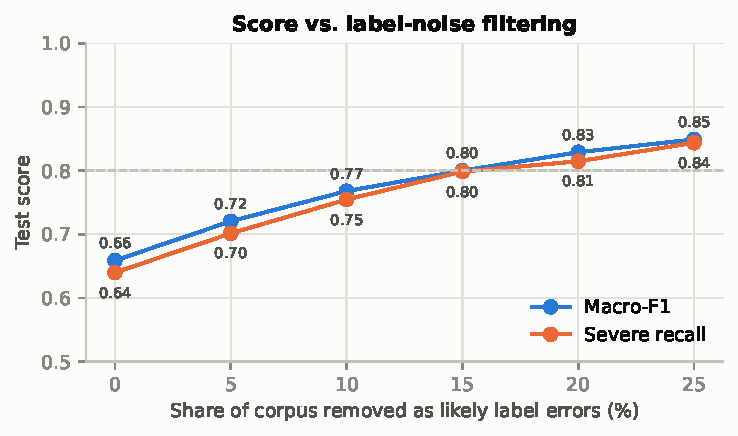
\includegraphics[width=0.9\linewidth]{fig7_noise_curve}
\caption{NB-SVM test macro-F1 and Severe recall when the given share of lowest-confidence posts is removed from the audited corpus before splitting. The dashed line marks 0.80.}
\label{fig:noise}
\end{figure}

\subsection{Severe Operating Point, Experiment E}

\begin{table}[!htbp]
\centering
\caption{Experiment E: Severe recall before and after tuning the Severe threshold for 0.80 out-of-fold recall on the training set, with Severe precision and macro-F1 after tuning.}
\label{tab:thr}
\begin{tabular}{lrrrr}
\toprule
 & \multicolumn{2}{c}{Severe recall} & & \\
Model & Before & After & Severe-P & Macro-F1 \\
\midrule
NB, BoW (A) & 0.703 & 0.772 & 0.592 & 0.629 \\
NB-SVM (C) & 0.640 & 0.791 & 0.636 & 0.651 \\
LR, TF-IDF (reference) & 0.677 & \textbf{0.823} & 0.602 & 0.637 \\
\bottomrule
\end{tabular}
\end{table}

Raising the weight of the Severe class (Table~\ref{tab:thr}) increases Severe recall by 7 to 15 points and costs 0.8 to 2.4 macro-F1 points. The TF-IDF LR reaches 0.823 Severe recall at 0.602 precision: it catches about 82 of every 100 Severe posts, and about 6 in 10 of its Severe flags are correct. NB-SVM reaches 0.791 with the best precision (0.636). For Naive Bayes, $\lambda$ hit the upper limit of 6 before the training target was met, because its probabilities sit very close to 0 or 1.

\subsection{Robustness over Five Splits}

\begin{table}[!htbp]
\centering
\caption{Mean $\pm$ standard deviation of test metrics over five stratified 80/20 splits (seeds 42 to 46), using each model's selected configuration.}
\label{tab:seeds}
\begin{tabular}{lrrr}
\toprule
Model & Macro-F1 & Severe-R & QWK \\
\midrule
NB, BoW & 0.652 $\pm$ 0.004 & \textbf{0.698 $\pm$ 0.009} & 0.561 $\pm$ 0.006 \\
LR, BoW & 0.611 $\pm$ 0.005 & 0.596 $\pm$ 0.005 & 0.500 $\pm$ 0.006 \\
RF, BoW & 0.624 $\pm$ 0.010 & 0.635 $\pm$ 0.013 & 0.539 $\pm$ 0.013 \\
NB-SVM, TF-IDF & \textbf{0.671 $\pm$ 0.008} & 0.644 $\pm$ 0.008 & \textbf{0.584 $\pm$ 0.011} \\
\bottomrule
\end{tabular}
\end{table}

All Experiment~A models vary by at most one macro-F1 point across splits (Table~\ref{tab:seeds}), so their ranking is stable. The TF-IDF LR reference is less stable: it scores $0.635\pm0.048$, and one split drops to 0.550. Its SAGA solver stops at 100 epochs before converging, and on that split the early-stopped solution is poor. The NB-SVM solver converges on every split, and its macro-F1 varies by only 0.008.

\subsection{Interpretability and Failure Cases}

\begin{figure}[!htbp]
\centering
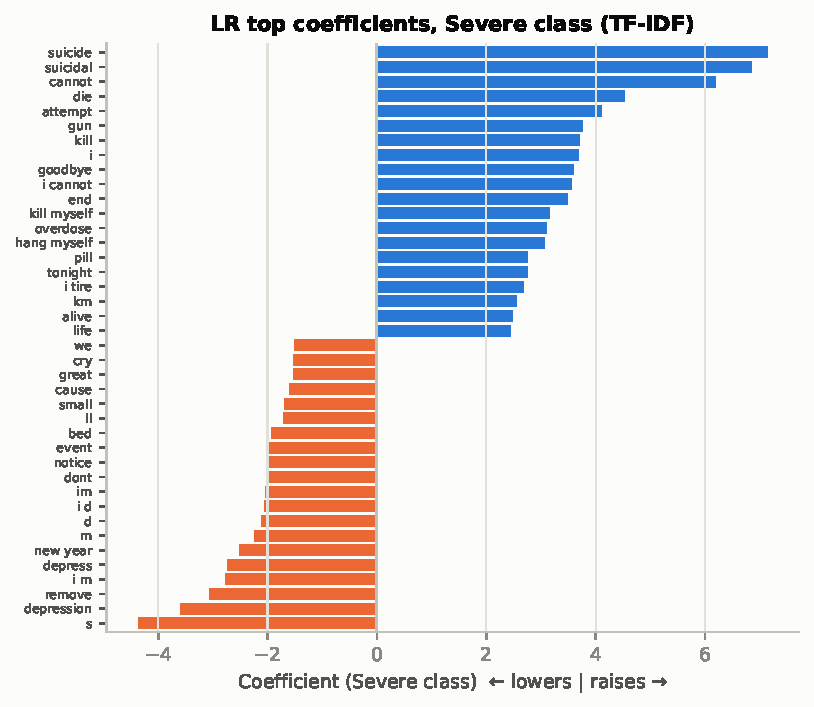
\includegraphics[width=1.0\linewidth]{fig3_lr_coefficients}
\caption{Largest positive and negative coefficients of the Severe class in the TF-IDF LR reference model. Positive coefficients push a post towards Severe.}
\label{fig:lr}
\end{figure}

\begin{figure}[!htbp]
\centering
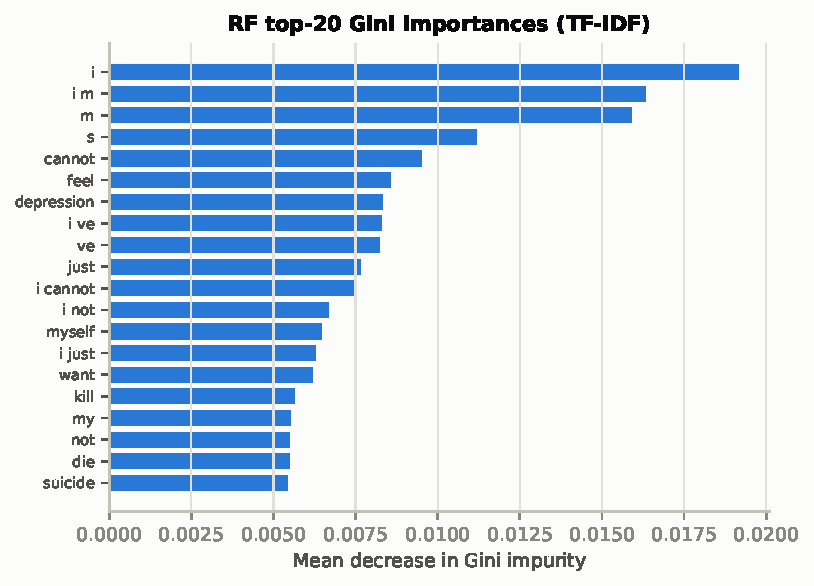
\includegraphics[width=1.0\linewidth]{fig4_rf_importances}
\caption{Top 20 Gini importances of the TF-IDF Random Forest reference model. Importance is the total impurity decrease from splits on the term.}
\label{fig:rf}
\end{figure}

For word-level interpretation we use the TF-IDF LR and RF reference models of Experiment~B. The L1 penalty gives zero weight in all four classes to 39.0\% of the LR vocabulary. The largest positive Severe coefficients (Fig.~\ref{fig:lr}) are suicidal-ideation and method terms (\textit{suicide}, \textit{suicidal}, \textit{die}, \textit{attempt}, \textit{kill}, \textit{gun}, \textit{goodbye}, \textit{kill myself}, \textit{overdose}, \textit{hang myself}, \textit{pill}, \textit{tonight}), together with the negation \textit{cannot}, the bigram \textit{i cannot} and the pronoun \textit{i}. A standard stop-word list would have removed three of the ten strongest Severe markers (\textit{cannot}, \textit{i}, \textit{i cannot}). RF importances (Fig.~\ref{fig:rf}) agree: \textit{i} is the most important feature, and \textit{cannot}, \textit{myself}, \textit{i cannot}, \textit{i not}, \textit{my} and \textit{not} are in the top 20 alongside \textit{kill}, \textit{die} and \textit{suicide}. Among the negative Severe coefficients, \textit{depression} and \textit{depress} suggest that posts discussing depression as a topic were annotated as milder than posts expressing intent, and terms such as \textit{new year}, \textit{remove} and \textit{event} look like artefacts of individual source corpora. The tokens \textit{m}, \textit{s} and \textit{ve} are left over from \textit{I'm}, \textit{'s} and \textit{I've}, which our preprocessing does not expand.

The models also fail in instructive ways. An illustrative sentence that we wrote, ``I cannot sleep anymore, I feel useless and hopeless and I just want to die'', is predicted Mild, because \textit{useless} and \textit{hopeless} carry Mild weight in this corpus: worthlessness contributes $+0.52$ and fatigue $+0.21$ to the Mild score, while \textit{die} adds almost nothing. The model reproduces the annotation habits of the corpus and does not check symptoms the way a clinician would.

\subsection{Computational Cost}

\begin{table}[!htbp]
\centering
\caption{Training time of one refit of the selected configuration and inference time per \num{1000} test posts, including vectorisation.}
\label{tab:time}
\begin{tabular}{llrr}
\toprule
Features & Model & Train (s) & Predict (ms / 1k posts) \\
\midrule
BoW & Naive Bayes & 1.7 & 44.5 \\
BoW & Logistic Regression & 231.8 & 53.6 \\
BoW & Random Forest & 50.1 & 216.7 \\
TF-IDF & NB-SVM & 5.6 & -- \\
\bottomrule
\end{tabular}
\end{table}

Naive Bayes trains in under 2~s and completes its grid search in under a minute (Table~\ref{tab:time}). RF needs about 50~s per fit with 500 trees, about 20 minutes per grid search on 4 cores, and is the slowest at inference (217~ms per \num{1000} posts against 45 to 54~ms for the linear models). LR is the most expensive to train: 232~s per fit and 58 minutes per grid search with BoW, because SAGA converges slowly under an L1 penalty, and its selected configuration stops at the 100-epoch limit. NB-SVM trains in 5.6~s.

% ---------------------------------------------------------------------------
\section{Discussion}

\textbf{Which model to use.} Naive Bayes on BoW gives the best Experiment~A macro-F1 (0.652) and Severe recall (0.703) and retrains in under two seconds, which makes it a strong default for a first-stage screener. NB-SVM is the strongest model overall ($0.671\pm0.008$) and is almost as cheap. Where catching Severe cases matters most, a tuned threshold trades about two macro-F1 points for Severe recall above 0.8, and LR remains the choice when a sparse, auditable list of weighted markers is required.

\textbf{The ceiling is in the labels.} A generative linear model, a discriminative linear model, a non-linear ensemble and NB-SVM all land between 0.60 and 0.67 macro-F1, and neither the lexicon nor training-label cleaning moves this by more than 0.6 points. Experiment~D shows why: about 19\% of posts carry labels that disagree with the rest of the corpus, mostly between Mild and Severe, and without them the same models reach 0.72 to 0.80. Larger models trained on the same labels are unlikely to remove this limit; re-annotating the inconsistent posts is more likely to help.

\textbf{The markers are plausible but narrow.} Explicit suicidal-ideation vocabulary drives the Severe class. This agrees with the clinical meaning of severe depression, but the models may miss severe depression expressed without such words. The weight of \textit{i}, \textit{cannot} and \textit{not} agrees with work on self-focus and absolutist language~\cite{rude2004language,almosaiwi2018absolute} and shows that stop-word choices made before training decide which signals survive.

\textbf{Audit before benchmarking.} The distributed file looks balanced only because Moderate posts were duplicated, and it contains contradictory labels. Neither problem shows in the class counts, and on the uncleaned file the model ranking reverses. Severity datasets assembled from several sources should report their de-duplication procedure and the corpus size after it.

% ---------------------------------------------------------------------------
\section{Limitations}\label{sec:limits}

The severity labels are text annotations aligned to BDI bands, not BDI scores collected from the authors of the posts, so the models learn to reproduce annotator judgements. The audit removes only the contradictions it can detect (identical text, different label); near-duplicates and inconsistent labelling across different texts remain. After preprocessing, 33 test posts (0.6\%) became identical to training posts because they differed only in case, punctuation or URLs; excluding them changes macro-F1 by at most 0.16 points and no ranking.

Experiment~D2 also removes test posts whose labels disagree with model predictions. Some of them may be hard but correctly labelled cases, so D2 scores estimate what consistent labels allow. The audited test set remains our main result, and we report both together with the share removed.

The corpus is English social-media text, so performance on clinical notes, other platforms or other languages is untested. BoW and TF-IDF ignore word order beyond bigrams and cannot resolve sarcasm, quotation or reports of another person's distress, and the DSAS lexicon matches keywords without handling negation (``I am not hopeless''). Only negative contractions are expanded, which leaves the fragments \textit{m}, \textit{ve} and \textit{s}. LR stops at 100 SAGA epochs, which makes the TF-IDF model unstable across splits, and the RF optimum lies on the edge of its grid. We checked robustness over five splits but ran no formal significance tests, so differences of about one macro-F1 point should not be over-interpreted. Gini importance favours frequent features~\cite{strobl2007bias} and L1 selection among correlated features is unstable, so both rankings show association, not causation.

% ---------------------------------------------------------------------------
\section{Broader Impact}

Automatic severity screening could help route people who write about distress towards support earlier and at low cost. The same technology can also harm. Inferring mental-health status from text is sensitive, false negatives can delay help for people at risk, and false positives can stigmatise. Any real use needs informed consent, data minimisation, human review of every Severe flag and a clear escalation path to crisis services. The models in this paper are screening aids that route people to professional assessment and must never be used as diagnostic instruments.

% ---------------------------------------------------------------------------
\section{Conclusion}

After removing the 29.9\% of the Depression Severity Levels Dataset that is duplicated or contradictorily labelled, classical models reach 0.65 to 0.67 macro-F1 on four-level severity classification. Naive Bayes on BoW is the best baseline (0.652, Severe recall 0.703), NB-SVM is the strongest model overall ($0.671\pm0.008$), and a tuned threshold raises Severe recall to 0.82. Severe predictions rest on suicidal-ideation terms, first-person pronouns and negation, so stop-word lists should be adapted rather than applied as they are. The DSAS lexicon published with the dataset adds no accuracy but explains predictions by symptom. On the uncleaned file, duplicates inflate LR and RF by more than six points and reverse the ranking, and setting aside the 19\% of posts with inconsistent labels lifts macro-F1 to about 0.80. Future work will benchmark transformer models on the same audited split, use ordinal or cost-sensitive losses that penalise Severe-to-Minimal errors most, and have clinical experts re-annotate the conflicting Minimal/Moderate posts and the posts flagged in Experiment~D.

\section*{Acknowledgment}
The authors thank the KUAS Ubiquitous Computing Lab for releasing the Depression Severity Levels Dataset openly.

\bibliographystyle{IEEEtran}
\bibliography{../refs}

\end{document}
